\documentclass[12pt,a4paper,twoside,english]{book}


\usepackage{Formato}


\title{Tesis 3 Estado del Arte }
\author{Aaron Sújar}

%%%%%%%%%%%%%%%%%%%%%%%%%%%%%%%%%%%%%%%%%%%%
%Nuevos comandos
%%%%%%%%%%%%%%%%%%%%%%%%%%%%%%%%%%%%%%%%%%%%
%\usepackage[normalem]{ulem}
%\usepackage{color}
%\usepackage[margin=2in]{geometry}
%\usepackage{todonotes}
\newcommand{\del}[1]{\textcolor{red}{\sout{#1}}} %\sout}
\newcommand{\new}[1]{\textcolor{blue}{\uline{#1}}} %\sout}


\begin{document}
\frontmatter


\pagenumbering{roman}

\thispagestyle{empty}
\chapter*{Acronyms}

\begin{acronym}
\acro{B-rep}{representación superficial}
\acro{Bangor}{Bangor University}
\acro{DQS}{dual quaternion skinning}
\acro{CAD}{diseño asistido por computador}
\acro{COR}{centros de rotación}
\acro{Courseware}{aplicación de entrenamiento}
\acro{DICOM}{Imagen y Comunicación Digital en Medicina}
\acro{DOF}{grados de libertad}
\acro{E/S}{Entrada/Salida}
\acro{EASA}{Agencia Europea de Seguridad Aérea}
\acro{FEM}{método de elementos finitos}
\acro{FORTH}{Foundation for Research and Technology - Hellas}
\acro{CGAL}{Computational Geometry Algorithms Library}
\acro{GLSL}{OpenGL Shading Language}
\acro{GMRV}{Grupo de Modelado y Realidad Virtual}
\acro{GPL}{GNU General Public License}
\acro{GPU}{unidad de procesamiento gráfico}
\acro{ITGVPH}{Integrated Toolkit for Generation of VPH Models}
\acro{INRIA}{Institut National de Recherche en Informatique et en Automatique}
\acro{IRM}{imagen por resonancia magnética}
\acro{joints}{articulaciones virtuales}
\acro{kvp}{tensión de pico}
\acro{LGPL}{GNU Lesser General Public License}
\acro{LBS}{linear blending skinning} 
\acro{MoCap}{captura de movimientos}
\acro{RA}{anestesia regional}
\acro{RAAs} {Regional Anaesthesia Assistant}
\acro{RAM}{Random Access Memory}
\acro{RASim}{Regional Anaesthesia Simulator}
\acro{RASimAs}{Regional Anaesthesia Simulator and Assistant}
\acro{RDT}{triangulación restringida de delaunay}
\acro{RV}{realidad virtual}
\acro{RWTH}{RWTH Aachen University}
\acro{SBS}{Spherical Blend Skinning}
\acro{SINTEF}{Stiftelsen for industriell og teknisk forskning}
\acro{SG}{Sensegraphics}
\acro{SOFA}{Simulation Open Framework Architecture}
\acro{TC}{tomografía axial computarizada}
\acro{TPTVPH}{Toolkit for Pose Transforms of VPH Models}
\acro{tracker}{dispositivo de seguimiento}
\acro{tabla hash}{Spatial Hash Table}
\acro{UKA-IMI}{Department of Medical Informatics: Uniklinik RWTH Aachen}
\acro{URJC}{Universidad Rey Juan Carlos}
\acro{US}{ultrasonidos} 
\acro{ViSTA}{Virtual Reality Toolkit}
\acro{VPH}{pacientes virtuales}
\acro{VTU}{formato de Visualization Toolkit}
\acro{WP}{paquetes de trabajos}
\acro{X3D}{formato Extensible 3D}
\acro{XML}{Extensible Markup Language}
\acro{ZPD}{zona de desarrollo próximo}


\end{acronym}



\tableofcontents
\listoffigures
 
\listoftables

\mainmatter
\chapter{Antecedentes} 
\label{cap:related}
\todo{
% Hay varias cosas en relación a la estructura de este punto que debes mejorar.
% Te planteo primero los problemas y luego una posible solcuicón:
% 1. No entiendo porque hablas de las la RA y de la radiolaogia diagnostica en le punto 1.1. 
% 2. No entiendo porque el punto 1.1.1 y el 1.3 están separados. 

Solución 
1.1 Simuladores Médicos de Realidad Virtual
1.1.1 Técnicas tradicionales (sin hablar de simuladores RV, lo que tengas pasaló al actual 1.1.3 )
1.1.2 Simuladores RV (Aquí va todo lo de G. Burdea)
1.1.3 Simuladores médicos (fusión de los actuales 1.1.1 y 1.3) cuando los fusiones que no te quede muy repetitivo. Vuelvelo a leer.
1.1.3.1 Aprendizaje (no me gusta mucho el título)
1.1.3.1 Evaluación. Mete validez dentro
1.2 Caracterización de los procedimientos simulados
1.2.1 RA
1.2.3 x-ray (los titulos antiguos)
1.3 RASimAs
1.4 Como está
}


En este capítulo se repasará la bibliografía que puede servir para ayudar al lector a comprender algunos conceptos ya introducidos y los que se introducirán en los capítulos siguientes. 
Además, se explicará en detalle la estructura del proyecto RASimAs, haciendo especial hincapié en las partes desarrolladas en este trabajo. El lector también podrá encontrar una revisión bibliográfica en la que se repasan los principales avances que se han producido en los últimos años en el área en la que se enmarca esta tesis, destacando sus fortalezas y debilidades. 

Se va a comenzar dando una perspectiva general de los simuladores de realidad virtual para luego centrarse en simuladores particulares de especial relevancia para el proyecto presentado. A continuación, se introducirá brevemente conceptos relacionados con el aprendizaje. También se detallará la evaluación a los que se someten los simuladores de realidad virtual, en concreto en el ámbito médico para probar su efectividad. \new{Posteriormente se introducirá al lector los procedimientos médicos en los que se ha trabajado en esta tesis. Además, se resumirá la división de tareas del proyecto \ac{RASimAs}. }
Por último, se introducirá al lector en el estado del arte en cuanto a las técnicas de animación de personajes dentro de la informática gráfica. Esta sección se centrará en describir las etapas de la animación esqueletal en las que está basado el algoritmo propuesto en esta tesis y las distintas propuestas que existen para automatizarlas y, por último, se compararán con los métodos de animación basados en modelos físicos.



\section{Simuladores de realidad virtual}
\label{art:simulador}

\begin{figure}[h]
   \centering
    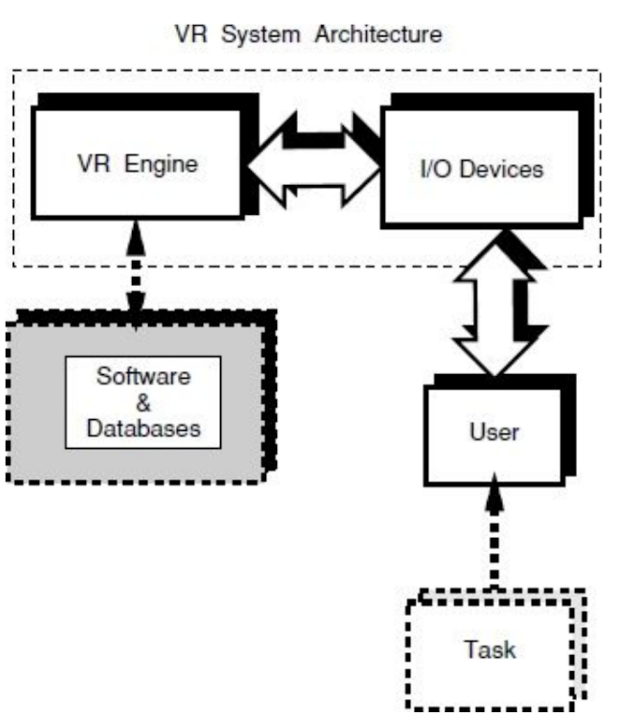
\includegraphics[width=0.5\textwidth]{IMG/VRarq.PNG}
    \caption{Arquitectura propuesta por \cite{burdea2003virtual} }
   \label{fig:RVarq}
\end{figure}
Según \emph{Burdea y Coiffet}\cite{burdea2003virtual}, un sistema de \ac{RV} se puede dividir en cinco componentes como se puede observar en la figura \ref{fig:RVarq}. En ella podemos observar las distintas interacciones que se producen entre componentes. De manera separada, estos componentes pueden existir independientemente pero es la relación entre ellos la que componen un sistema \ac{RV}. A continuación se describirá cada uno de ellos:
\begin{itemize}
    \item Motor de \ac{RV}: Este componente se encarga de realizar los cálculos necesarios para simular la escena virtual. Para actualizar el estado de la escena virtual, es necesario que consulte las bases de datos y software incluidos en el sistema y actuará según la entrada recibida a través de los dispositivos realizada por los usuarios. El motor generará y mostrará el nuevo estado de la escena a través de los dispositivos de salida (que pueden incluir más de un canal sensorial). Además, es preciso asegurar una tasa interactiva al realizar estos cálculos. Este término se tiene que tratar como una abstracción ya que puede tener múltiples configuraciones hardware como puede ser un computador o un sistema distribuido conectado por red.
    \item Dispositivos de \ac{E/S}: Este componente se basa en todos los dispositivos que utilice el usuario en su interacción con el sistema. Es imprescindible en un sistema \ac{RV} permita la interacción del usuario. Los dispositivos de entrada se encargan de recoger las acciones que realiza el usuario, y recibe la respuesta de la escena virtual a través de los dispositivos de salida de los distintos canales sensoriales. Estos dispositivos son muy numerosos y diversos actualmente.
    \item Componentes software y base de datos: Este módulo contiene todas las especificaciones y descripciones que caracterizan el sistema y la escena virtual. Aquí se incluyen la escena virtual y su organización que es consultada por el motor de \ac{RV} análogamente a lo que correspondería como una base de datos, donde se consulta y se recoge la información necesaria para la simulación. Además, aquí se incluyen, por ejemplo, las aplicaciones que se diseñan con el objetivo de guiar y facilitar el entrenamiento al dirigir la simulación según la interacción del sistema y el usuario.
    \item Usuario: Es natural que los sistemas se diseñen con el objetivo de que una persona interaccionará y espera una respuesta en forma de estímulos a través de los dispositivos de \ac{E/S}. 
    \item Tareas: Por último, son las tareas, objetivos e instrucciones que se le dan al usuario cuando va a utilizar el sistema \ac{RV} que le dan significado y utilidad al simulador. Es lo que le diferencia de ser un computador con periféricos conectados de una plataforma de entrenamiento para pilotos o médicos. 
    
\end{itemize}

Esta definición de arquitectura será utilizada en el capítulo \ref{cap:rasim} como apoyo para explicar el simulador \ac{RASim} y sus diferentes componentes. A su vez, también puede ayudar al lector a hacerse una idea de como se 





\subsection{Simuladores para formación médica}
\label{art:medicalsim}

En los últimos años, los simuladores médicos de realidad virtual están tomando una gran importancia en el currículum de los estudiantes, como pueden ser los cirujanos y otras especialidades \cite{PATEL2017266.e7}. Se puede observar un incremento de su presencia para el entrenamiento de jóvenes especialistas tanto en hospitales como universidades. Estas herramientas proporcionan al usuario un método seguro y efectivo de entrenamiento, siendo capaces de usarlo tantas veces como sea posible. 

Aun con la introducción de los simuladores, todavía el entrenamiento médico se basa en una variedad de técnicas que permite al médico adquirir las destrezas necesarias antes de poder enfrentarse a escenarios reales de manera autónoma. Una forma segura de entrenamiento es la utilización de \emph{fantomas}\cite{phantomra}. En la figura \ref{fig:phantom} se puede ver un maniquí \emph{Blue Phantom™}\cite{BluePH}.

\begin{figure}[h]
   \centering
    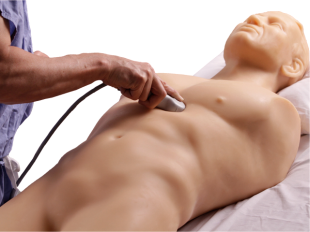
\includegraphics[width=0.5\textwidth]{IMG/fast_trauma.jpg}
    \caption{Maniquí realista para el entrenamiento de ultrasonidos \emph{Blue Phantom™}\cite{BluePH} }
   \label{fig:phantom}
\end{figure}

Estos \emph{fantomas}\footnote{castellanización del término inglés Phantom} son modelos anatómicos hechos con materiales sintéticos intentando replicar el cuerpo humano fielmente y sus propiedades. En ocasiones, tienen incorporados una serie de sensores que permiten recogida de métricas. A pesar de que son muy populares, tiene una serie de inconvenientes: no son baratos, y suelen ser creados específicamente para una zona anatómica concreta, no siendo posible usarlos en otras circunstancias para lo que fueron creados. Además, si en determinadas ocasiones, el usuario tiene que manipularlos como puede ser hacer una incisión o inyección en el \emph{fantoma}, el modelo sufre desgaste con el tiempo.

Otra forma de entrenamiento es la utilización de cadáveres\cite{Tsui2007}, que permiten una anatomía real muy alejada de los muñecos poco realistas. En este caso, conseguir diferentes variaciones anatómicas es completamente viable y el mismo cadáver puede servir para entrenamientos de diferentes procedimientos. Aun así, los inconvenientes que presentan son bastante evidentes. Mantener un cadáver en buenas condiciones y que los motivos del fallecimiento perjudiquen al estado del mismo, son los principales problemas que nos encontramos además de ciertos problemas éticos como puede ser el uso de cadáveres procedentes de condenados a pena de muerte como puede ser el Visible Human Project \cite{ackerman1998visible}. Introducir sensores o algún tipo de dispositivo que permitan evaluar el rendimiento tampoco es sencillo. Finalmente, los tejidos de un cadáver no muestran el mismo comportamiento mecánico que un paciente, y puede inducir sesgos en el entrenamiento del médico debido a que los músculos se vuelven más rígidos después del fallecimiento.


La última forma de entrenamiento es el entrenamiento sobre pacientes reales, donde al estudiante realiza el procedimiento supervisado y guiado por su tutor. Aunque es el entrenamiento más realista, obviamente incluye una serie de riesgos y situaciones no controladas que pueden ser peligrosas para el paciente.


A diferencia de los métodos anteriormente citados, los simuladores de realidad virtual permiten un entrenamiento más barato y rápido donde los estudiantes pueden mejorar sus habilidades. Mejoras en el rendimiento, nuevos dispositivos periféricos y desarrollo de nuevas técnicas de simulación física permiten una transferencia efectiva de habilidades del mundo virtual al mundo real, como podemos observar a continuación.
Habitualmente los simuladores  son específicos de cada procedimiento médico donde podemos encontrar un simulador de cirugía ortopédica \cite{cecil2017advanced}, o por ejemplo un simulador de cirugía cardiovascular \cite{korzeniowski2018vcsim3}. Incluso, podemos incluir diferentes tipos de simulación, donde \cite{villard2014interventional} es un simulador de radiología intervencional donde además de entrenar la habilidad manual, es necesario aprender como guiar la aguja a través de imagen de rayos X.

Pero además, la nueva generación de simuladores no solo se centran en mejorar la calidad de la simulación, sino que también quieren permitir el entrenamiento con datos de pacientes reales\cite{Willaert2012,  Votta2013}. 






\subsection{Diagnóstico por imagen médica}
\label{art:xraysim}

En radiología, la forma más común de aprender diagnóstico por imagen son los archivos educativos. Son recopilaciones de imágenes médicas de pacientes reales acompañados normalmente del historial del paciente. En estos archivos, los estudiantes pueden buscar a través de la gran cantidad de casos bien documentados. Normalmente, cada universidad, hospital o facultad tienen sus propios repositorios, incluso existen libros que se pueden consultar como \cite{carver2012medical}.
En la última década, cada vez más se publican estos recursos de manera online donde cualquier radiólogo pueda consultar un enorme base de datos de imágenes de cualquier parte de la anatomía humana \cite{deshpande2017integrated}. 

Actualmente, la educación se ha visto beneficiada por la incorporación de los teléfonos inteligentes en este ámbito. Algunas instituciones han creado aplicaciones donde los estudiantes pueden revisar e investigar los casos almacenados, realizar cuestionarios y mejorar el aprendizaje como es el caso de la aplicación \emph{UBC Radiology} \cite{Spouge2017}. Estos recursos se encuentran muy presentes en el aprendizaje de los radiólogos noveles, pero todos estos recursos mantienen el mismo problema. Las imágenes registradas son estáticas, y la mayoría de estas imágenes corresponden a imágenes que se presuponen que son correctas y no muestran ningún tipo de fallo. Esto es completamente entendible, ya que al hacer este tipo de recursos se seleccionan para intentar ser educativos. Además, ninguna imagen es del mismo paciente en diferentes situaciones o partes del cuerpo por razones de seguridad. Aun así, posicionar bien al paciente mientras se realiza el diagnóstico por imagen es algo imprescindible y algo necesario que el estudiante domine.

Mejoras en el rendimiento de los computadores permiten crear nuevos simuladores que mejoran y reducen el tiempo de aprendizaje de los estudiantes. Un caso remarcable es el  ProjectionVR$^{TM}$ \cite{shanahan2016student}. Este simulador trata de introducir al usuario dentro de un entorno realista 3D que quiere replicar una sala de rayos X para simular el procedimiento completo. Con datos de pacientes reales digitalizados, el simulador replica un entorno de aprendizaje sin el consecuente riesgo de radiación que significaría exponer a los estudiantes o los pacientes. Aunque provee una cantidad amplia de datos médicos, los datos que contienen son estáticos y los usuarios no pueden variarla o modificarla en el simulador. 

%https://www.bluephantom.com/product/Sciatic-Nerve-Regional-Anesthesia-Ultrasound-Training-Model.aspx?cid=428


\subsection{Anestesia regional}

Como se ha comentado con la anterior sección, existen multitud de simuladores dependiendo de su procedimiento médico que se pretende simular. En cuanto a la especialidad de anestesiología, la anestesia espinal y la epidural son los dos ejemplos más frecuentes dentro de la anestesia regional y podemos encontrar simuladores específicos \cite{broom2018evaluation}. Sin embargo, la búsqueda de un simulador de anestesia regional genérico es más complicada. Energid Technologies ha desarrollado  un simulador en un contrato con el Ejército de Estados Unidos, pero no ha sido comercializado al público \cite{lim2008simulation}.

Otro simulador, en este caso comercial, llamado SAILOR es distribuido acompañado de un atlas multimedia de los bloqueos de nervios. Este simulador presenta solo un único modelo de paciente, y su interacción es exclusivamente con el ratón sin ninguna tipo de deformación del tejido. \cite{Bibin}

En un estudio previo al proyecto RASimAs, se demostró la aceptación que tendría un simulador para la anestesia regional. Todos los participantes se mostraron muy receptivos con el trabajo realizado, sin embargo, se pudo constatar la escasez de nervios para bloquear, la pobre simulación de los ultrasonidos y una respuesta háptica realista \cite{Grottke2009594}.

%https://www.gtsimulators.com/Full-Body-X-Ray-Phantom-with-Real-Human-Skeleton-p/ez7200.htm
\subsubsection{RASIMAS}
\label{art:rasimas}

\todo{ es importante que describas la RA y la Radiología diagnostica en el estado del arte. Deben ir los pasos detallados del procedimiento. Pon alguna cita en el estado del arte. Por ejemplo, el CV de RA de Cork. Esto luego lo usaras en el courseware}

La \acl{RA}(\acs{RA}) guiada por \acl{US}(\acs{US}) representa una alternativa a la estimulación eléctrica. Las ventajas de utilizar una imagen de \ac{US} solventa las debilidades de la técnica tradicionalmente prácticada. La principal ventaja es la posibilidad de confirmar la propagación del anestésico alrededor del nervio objetivo. Además de la posibilidad de observar la aguja y el nervio, la imagen revela todas las estructuras internas como fascias, pleura, e incluso tejidos delicados como los vasos sanguíneos. 

\begin{figure}[h]
   \centering
    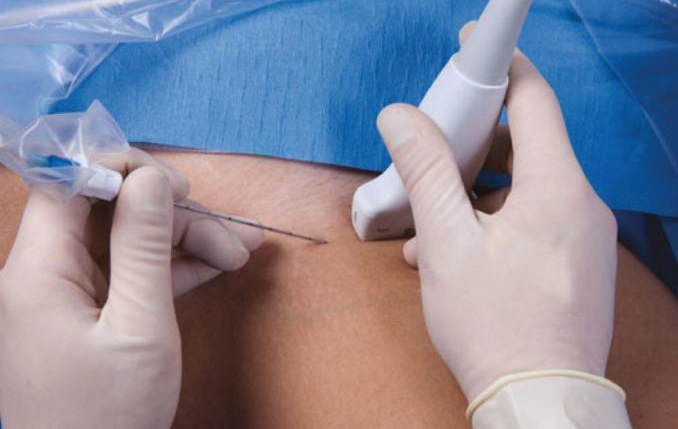
\includegraphics[width=0.5\textwidth]{IMG/RAUS.png}
    \caption{ Anestesia regional guiada por \acl{US}}
   \label{fig:raus}
\end{figure}

La ejecución de este procedimiento no es sencillo para aquellos profesionales de anestesiología que no están familiarizados con las técnicas de \ac{US}. Además de los conocimientos teóricos, los profesionales deben entrenar sus habilidades no cognitivas. Estos entrenamientos habitualmente se practican con paciente reales, con la utilización de cadáveres\cite{Tsui2007} o el uso de \emph{fantomas}\cite{phantomra}. La incorporación de un simulador en el entrenamiento del procedimiento ayudará a solventar las limitaciones de los entrenamientos clásicos al ser más barato, repetible y seguro.

El proyecto \ac{RASimAs} tiene como objetivo \new{el} de facilitar el entrenamiento y la práctica de la \ac{RA} con la ayuda de un simulador (\ac{RASim}) y un asistente (\ac{RAAs}).
Para que sea utilizado en el mayor número de sitios posibles (hospitales, universidades y colegios profesionales) se debe proporcionar una herramienta de entrenamiento que sea barata, fácil de usar, robusta y que necesite poco mantenimiento.
Estas herramientas están dirigidas para diferentes perfiles de usuarios.  Tanto estudiantes como profesionales que están empezando a realizar el procedimiento, el simulador les proporcionará un método de entrenamiento con el que mejorar sus habilidades cognitivas y propioceptivas. A su vez, este proyecto también está orientado para profesionales anestesistas que han estado alejados de la práctica del procedimiento y quieran retomar la actividad.
Los objetivos principales del simulador \ac{RASim} son los siguientes:
\begin{enumerate}
    \item Un estudiante de \new{anestesista} \del{anestesista} adquiera y desarrolle las habilidades cognitivas y no cognitivas que le permitan ejecutar un bloque de nervio guiado por \ac{US} empezando por el bloqueo del nervio femoral y siguiendo con las siguientes localizaciones.
    \item Permitir a un anestesista retomar y practicar las habilidades necesarias para realizar el procedimiento de forma segura y satisfactoria.
    \item Recuperar y medir métricas de rendimiento al realizar el procedimiento en el simulador. 
    \item Permitir a un supervisor revisar las métricas registradas por los usuarios del simulador a través del tiempo
\end{enumerate}



Según (entregable 2.1 \cite{rasimasweb}), el procedimiento de \ac{RA} guiado por \ac{US} se puede definir con los siguientes bloques:
\begin{enumerate}
    \item Exploración (\emph{Scout Scan}): El profesional configura y explora con la sonda de \ac{US} la zona del paciente con el objetivo de identificar el nervio, la arteria principal y las demás estructuras importantes (figura \ref{fig:scoutscan}). 
\begin{figure}[th]
   \centering
    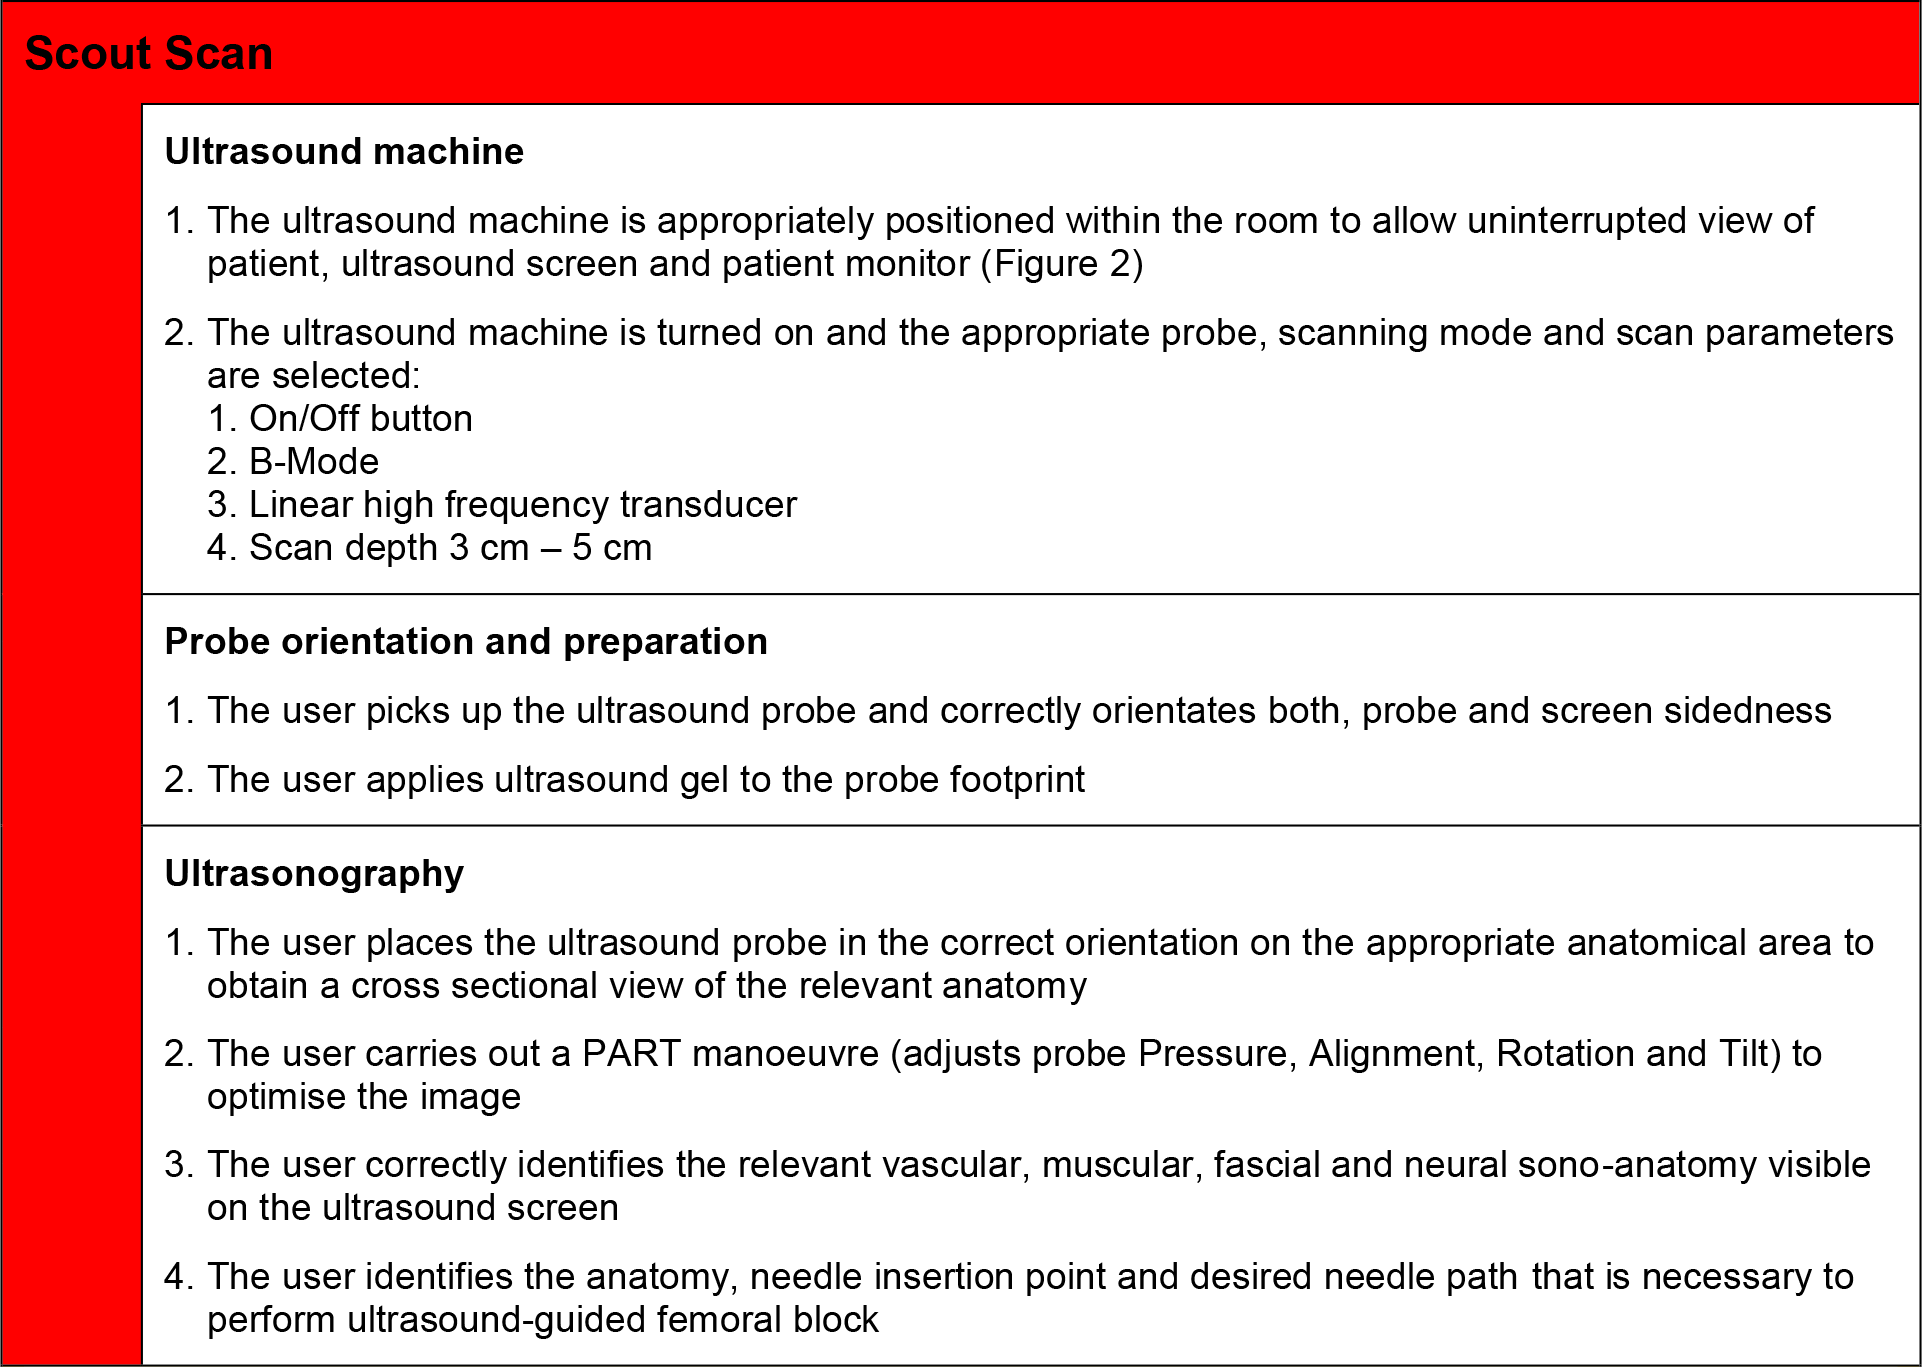
\includegraphics[width=0.9\textwidth]{IMG/scoutscan.png}
    \caption{Tareas del bloque de exploración }
   \label{fig:scoutscan}
   
\end{figure}
\todo{ Las imágenes se ven fatal, las paso a word, word a pdf y las pongo en el anexo? puedo citarlas también en los resultados}
    \item Guiado de la aguja (\emph{Needle Guidance}): A partir de que se ha interpretado la imagen de \ac{US}, el profesional guía la aguja a través de la anatomía hasta el nervio (figura \ref{fig:needleguidance}).  
    \begin{figure}[th]
   \centering
    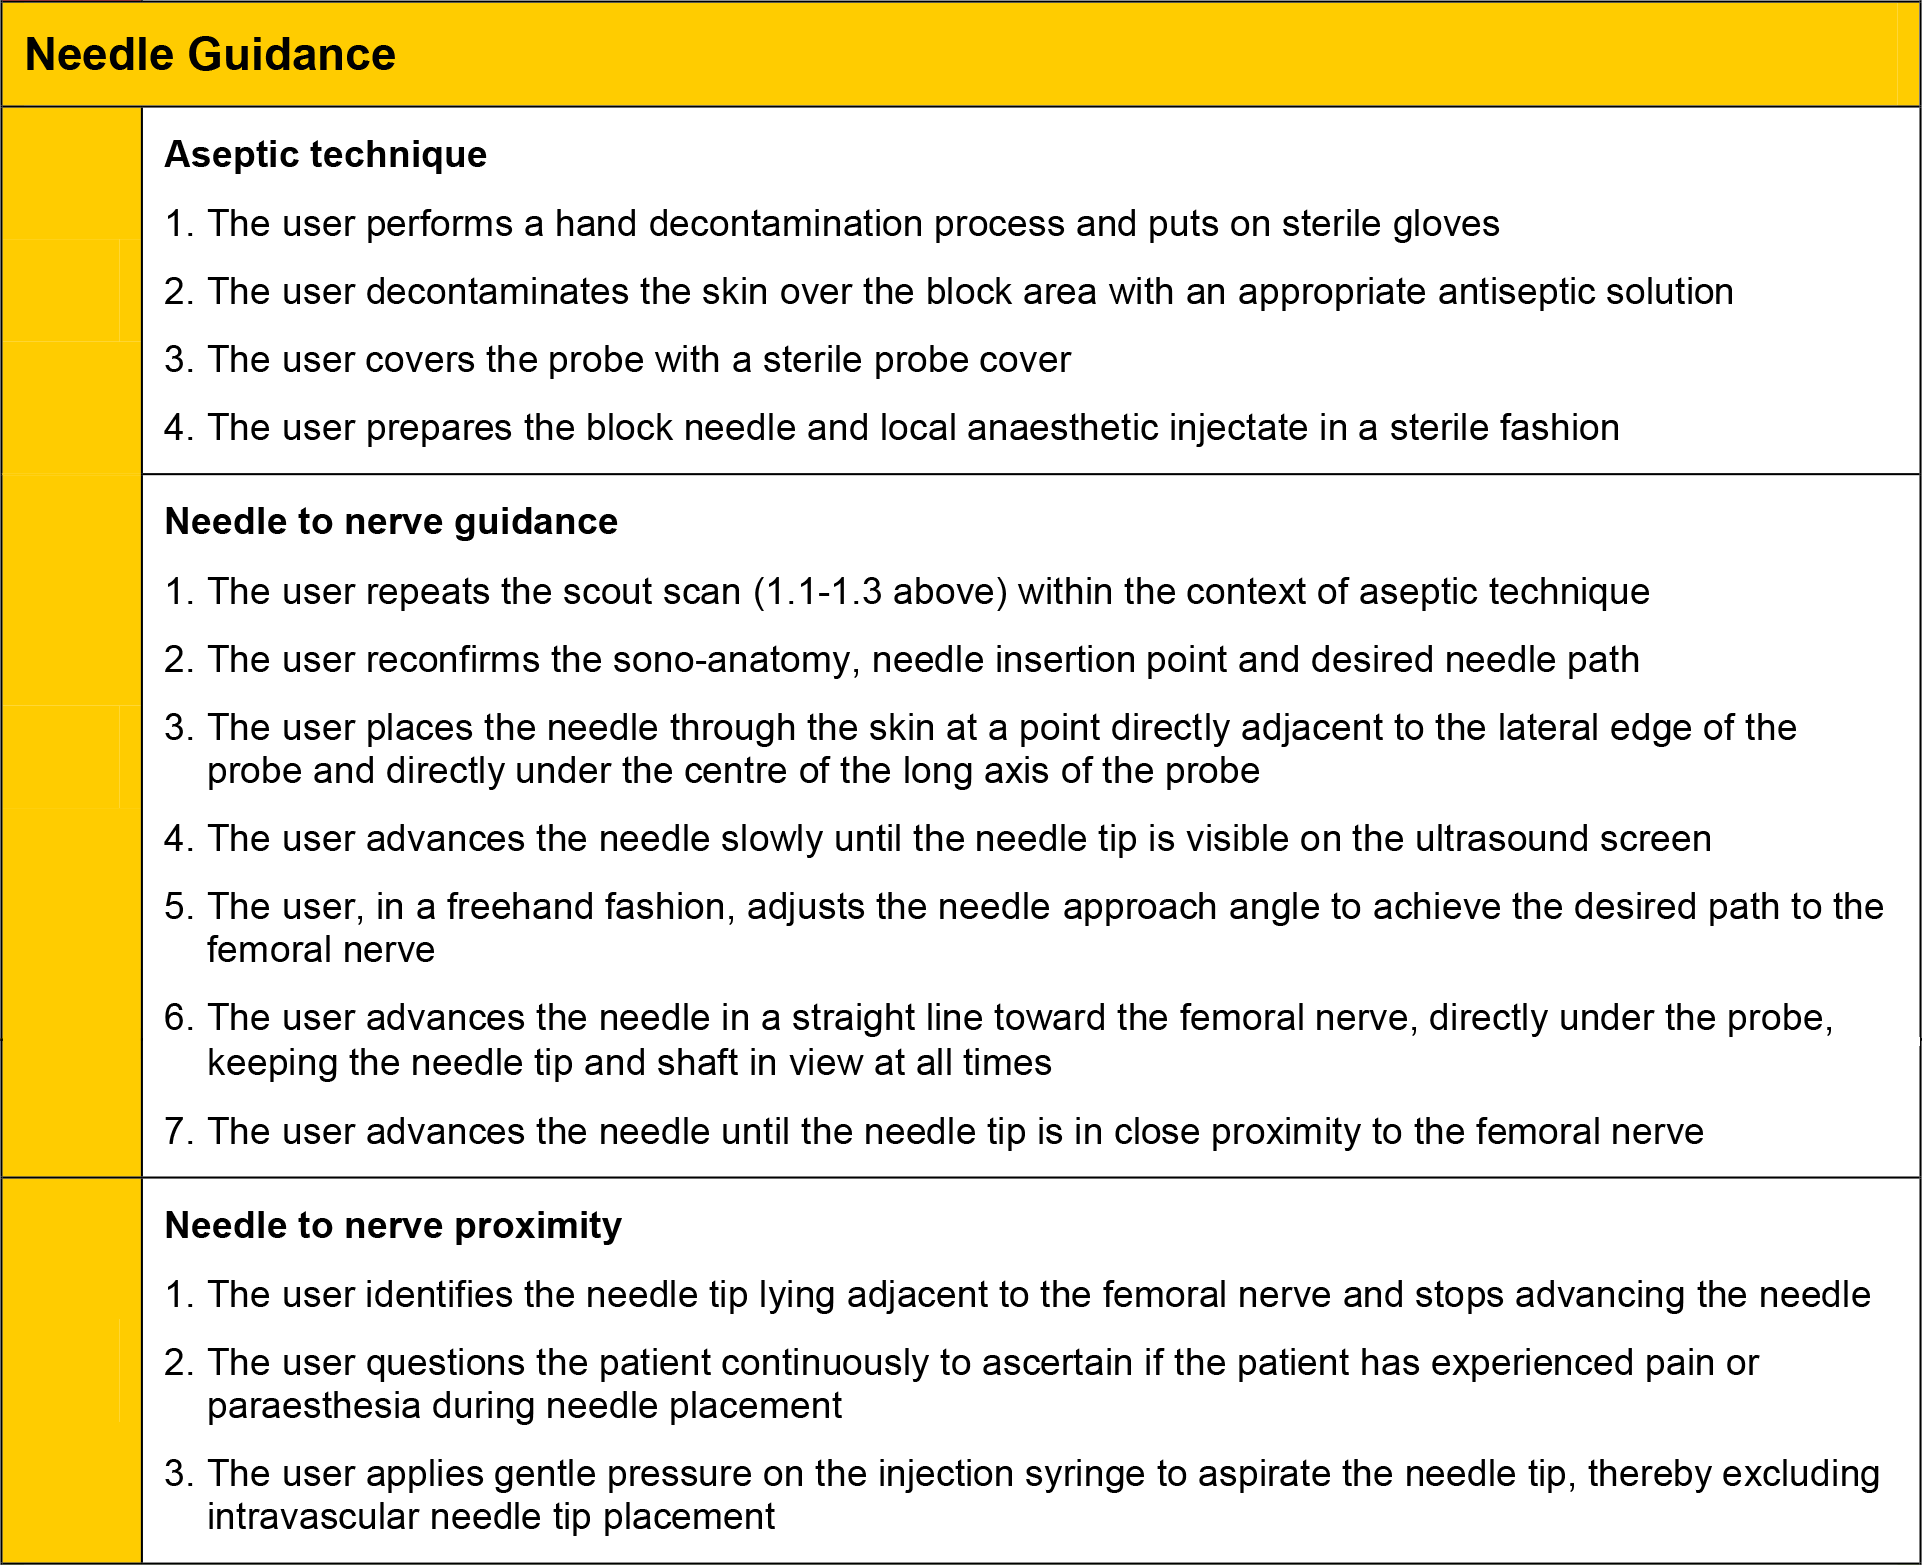
\includegraphics[width=0.9\textwidth]{IMG/needleguidance.png}
    \caption{Tareas del bloque de guiado de la aguja. }
   \label{fig:needleguidance}
\end{figure}
    \item Inyección (\emph{Injection}): El médico libera el bolo y confirma la correcta realización del bloqueo del nervio (figura \ref{fig:injection}). 
    \begin{figure}[th]
   \centering
    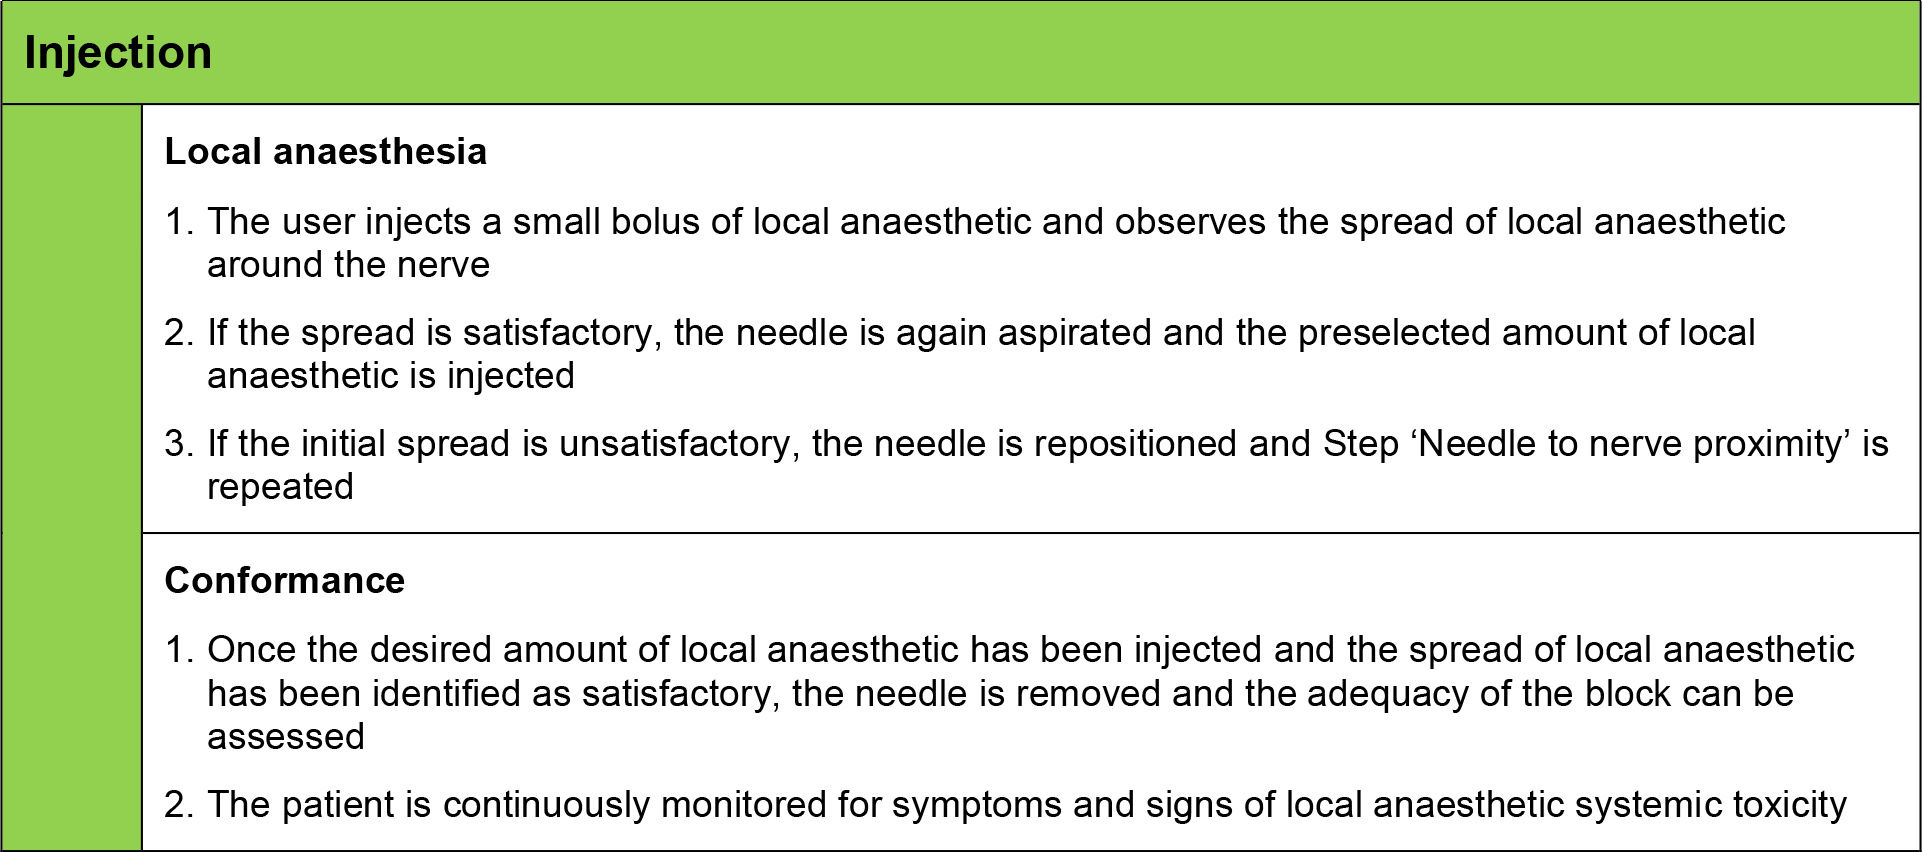
\includegraphics[width=0.9\textwidth]{IMG/injection.png}
    \caption{ Tareas del bloque de inyección.}
   \label{fig:injection}
\end{figure}
\end{enumerate}

Con el objetivo de explicar detalladamente cada bloque, se resumirá a continuación el procedimiento completo:

El anestesista deberá posicionarse en la sala de tal forma que su ángulo de visión permita observar el paciente, y el monitor de \ac{US} y de las constantes vitales sin mover la cabeza (figura \ref{fig:roomplace}). El médico configurará el equipo de \ac{US} con los valores apropiados, y explorará la zona anatómica con la sonda. Para conseguir una imagen adecuada para identificar los tejidos, se procederá a la maniobra PART (del inglés \emph{Pressure, Alignment, Rotation and Tilt}) que permite colocar correctamente la sonda de \ac{US} para asegurar una buena imagen donde se puedan localizar todas las estructuras importantes. Una vez el nervio esté localizado, el médico introducirá la aguja en plano\footnote{La aguja se introduce en paralelo con la proyección ultrasonográfica para que quede totalmente visible en la imagen.} con la sonda de \ac{US}, permitiendo así su visualización en la imagen y la dirigirá hasta la proximidad del nervio. Es entonces cuando, antes de inyectar el bolo, deberá aspirar primero para comprobar que la punta de la aguja no se encuentre dentro de un vaso sanguíneo y pueda causar toxicidad sistémica \footnote{El anestésico se distribuirá por los vasos sanguíneos.}. Una vez comprobado, a continuación solo se distribuirá una pequeña cantidad para asegurarse de la localización de la aguja y por último se liberará el bolo completamente. El profesional deberá confirmar que el bloqueo ha sido satisfactorio y comprobará cualquier síntoma de malestar en el paciente.


\begin{figure}[th]
   \centering
    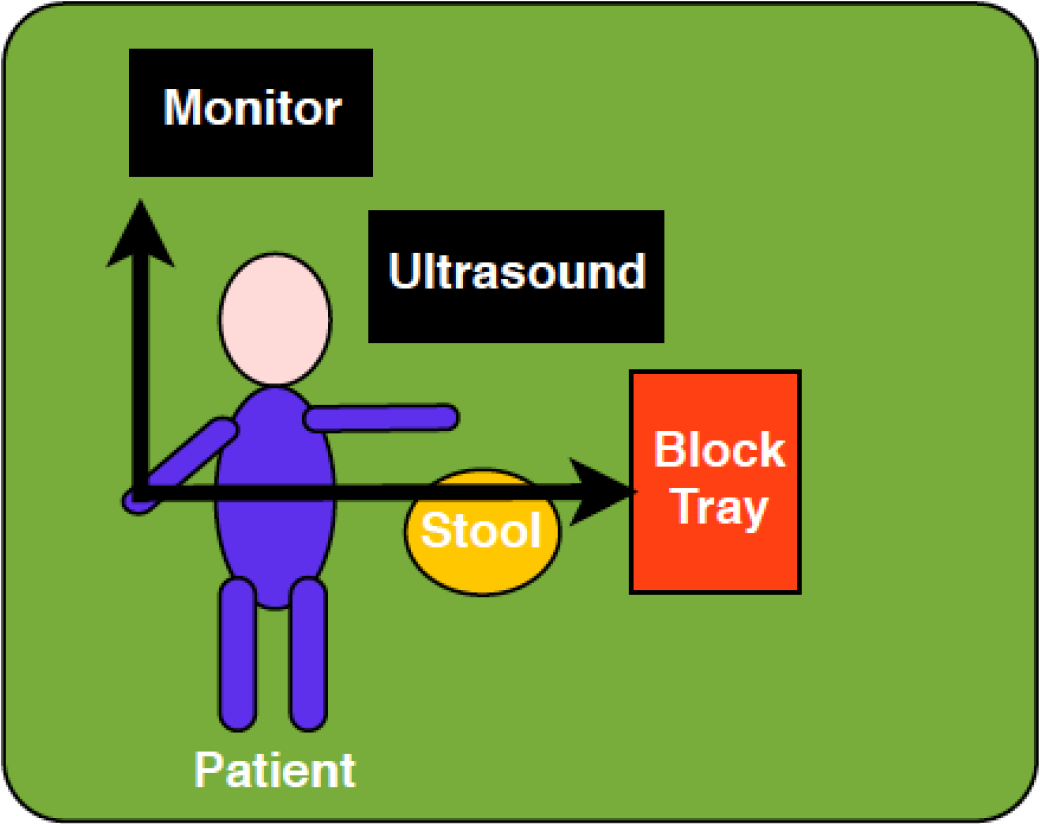
\includegraphics[width=0.5\textwidth]{IMG/roomplacement.png}
    \caption{ }
   \label{fig:roomplace}
\end{figure}




%\subsubsection{Objetivos del simulador}


% 6.1.3 Principles of use
% 1. RASim must be contextually relevant and function within the existing or evolving regional
% anaesthesia curriculum
% 2. RASim training must be based upon appropriately detailed characterised procedures
% 3. RASim training must allow the development of relevant procedural skills and associated
% clinical decision making
% 4. RASim training must never allow the development of procedural skill relevant only within
% the simulation environmentRASim training should allow performance related feedback, repeated practice and
% performance tracking and progression over time each based on precisely defined metrics
% 6. RASim based training programmes must have a defined beginning and end (entry and
% exit) constituting proficiency based progression for defined applications e.g. independent
%practice , supervised practice


\section{Entrenamiento con simuladores médicos}
\label{art:learning}


%En anteriores secciones se ha revisado el uso de simuladores en medicina aunque es bien sabido que el uso en otro tipo de contextos no es nuevo. El principal objetivo de estos simuladores es garantizar la seguridad e intentar mejorar el aprendizaje y la respuesta antes errores poco comunes.

En \cite{donaldson2000err} se cifra en cientos de miles las muertes ocurridas en hospitales estadounidenses como consecuencia de errores médicos, eso sin contar posibles otro tipo de daños a los pacientes que implican gastos económicos. En este libro se planteaba la necesidad de mejorar la formación de los profesionales para evitar este tipo de errores. 
Es necesario también garantizar la seguridad y la intimidad de los pacientes durante el proceso de aprendizaje, lo cual lleva implícito la exigencia ética que representa el propio código deontológico del personal sanitario. 

En el libro \cite{dent2017practical} se presenta una serie de objetivos que debería cumplir una institución de enseñanza médica al formular el currículum del personal sanitario.
\begin{itemize}
    \item Producir nuevos profesionales sanitarios.
    \item Utilizar los procedimientos médicos modernos.
    \item Cumplir la regulación gubernamental.
    \item Asegurar que los estudiantes puedan completar el curso.
    \item Satisfacer las expectativas de los pacientes.
\end{itemize}

Estos objetivos se enfrentan con una serie de problemas que han impulsado a las instituciones médicas a potenciar el uso de los simuladores.
Por una parte,  desde hace décadas se vienen disminuyendo el tiempo de trabajo para los profesionales en formación, que a la vez reduce el tiempo con pacientes reales. Además,  ha habido cambios respecto a que un paciente sea objetivo de exploraciones y procedimientos redundantes con objeto de entrenar a estudiantes, siendo una molestia y constituyendo un peligro. También hay que añadir que movimientos por los derechos de los animales han hecho restringir el uso de estos con motivos de aprendizaje. Por otra parte, ciertas organizaciones han cambiado sus métodos de evaluaciones con acreditaciones y certificaciones frente a la clásica evaluación basada en el conocimiento exclusivamente.

Otro motivo por el cual es necesario cambiar las formas de aprendizaje de la medicina, es debido a que estas también han evolucionado con el tiempo.
Tradicionalmente, el plan de estudios de la medicina era incremental desde los aspectos más básicos hasta llegar a la especialización. Actualmente la medicina es tan extensa que el contenido del currículum se ha incrementado notablemente. Esto ha hecho que aparecieran escuelas para cada especialidad médica donde el conocimiento médico ha crecido exponencialmente en las últimas décadas y los métodos tradicionales de enseñanza no son completamente adecuados para manejar esa cantidad de material.

Obligados a buscar alternativas para garantizar una exposición clínica variada y completa, junto con el desarrollo de la investigación en el campo de la simulación, los simuladores de \ac{RV} están aumentando su presencia dentro de los procesos de aprendizaje de los futuros médicos.

Por consiguiente, los simuladores se han mostrado como métodos adicionales de enseñanza frente a los métodos tradicionales. Estas nuevas formas de aprendizaje deben ser validadas antes de su incorporación definitiva. A continuación, primero se comentarán una serie conceptos básicos de aprendizaje que han de tomarse en cuenta en el desarrollo y diseño de una herramienta de entrenamiento. Posteriormente, se presentarán los instrumentos habituales que se utilizan para probar y validar de forma objetiva estas herramientas.


\subsection{Aprendizaje}

Frente a un modelo asistencial en la formación de los estudiantes, los simuladores presentan  ventajas educativas que convierten estas herramientas en ideales para enfrentarse a los problemas anteriormente citados. Estas herramientas han demostrado que pueden reducir el tiempo de realización de una tarea, así como el número de errores cometidos y, además, siendo posible diferenciar entre expertos y novatos \cite{Gurusamy08}.

Por otra parte, los simuladores permiten que el estudiante cometa errores sin las consecuencias reales que podrían resultar en un entorno con pacientes. El alumno se puede enfrentar a todo tipo de situaciones, desde las introductorias a las más complicadas donde errar no es crítico. También permite que el alumno reciba valoraciones y comentarios en tiempo real. Citando a \cite{ziv2008educacion}: "Los errores son experiencias de aprendizaje y ofrecen grandes oportunidades de mejorar a través del aprendizaje de los mismos". Adicionalmente, los simuladores presentan un entorno educativo estandarizado, reproducible y objetivo que permite una evaluación del estudiante constante.

% Según \cite{pales2010uso}hay una serie de condiciones que van son necesarios para que los simuladores sean un método eficaz de enseñanza.

% \begin{itemize}
% \item Los simuladores se tienen que basar en una planificación estricta junto con los objetivos docentes. Deben tener un guión que refleje claramente la situación a simular, los objetivos marcados y las competencias que se van a entrenar.

% \item Las habilidades entrenadas tienen que estar integradas en el currículum  y se debe planificar la enseñanza de diferentes habilidades complementariamente a la enseñanza teórica. Lo que se enseña debe ser relevante en el contexto

% \item La evaluación es una parte esencial del proceso como en cualquier otra actividad educativa. La retroalimentación es una de las partes imprescindibles de la simulación
% \item Cualquier simulador no puede estar aislados del entorno clínico real y se debe ser consciente de sus limitaciones y de las limitaciones de la tecnología. El manejarse correctamente con el simulador no es igual a competencia clínica.
% \item Los usuarios deben ser conscientes de que aunque trabajan en un entorno de simulación, han de actuar de la misma manera como lo harían en la realidad. El material de simulación no puede considerarse como un mero juguete y en su manejo han de observarse las mismas condiciones de uso y seguridad que en la realidad.

% \end{itemize}



%Sofia says:
%Deliberate Practice and the Acquisition and Maintenance of Expert Performance in Medicine and Related Domains Ericsson, K Anders
%Deliberative practice «Ericsson»( practicar muchas horas no es suficiente, hay que practicar fijándose en las cosas a reforzar y en lo que hay que mejorar... y se requieren un número mínimo de horas para llegar a convertirse en experto, estas horas siempre va ser más barato entrenarlas con un simulador, una vez adquirido y descontado el coste inicial, por lo que un simulador es interesante cuando mucha gente la practicar muchas horas).

Los simuladores no basan su eficiencia en la posibilidad de entrenar muchas horas, sino en cómo se entrena. Según \emph{Ericsson et al.} \cite{ericsson1993role}, la práctica de una misma habilidad durante un periodo largo de tiempo no es suficiente para llegar a ser un profesional, sino que es necesario enfocar de forma distinta los entrenamientos que simplemente repetir una y otra vez el ejercicio. \emph{Ericsson et al.} comenta que es necesario cambiar de enfoque y practicar fuera de la zona de confort. Además, también hace hincapié que la falta de una adecuada retroalimentación hace imposible un aprendizaje eficiente y no se producirán mejoras aunque los sujetos estén motivados. La motivación es algo fundamental en el entrenamiento, pues sin ella, el aprendizaje se ve ralentizado e incluso ser contraproducente. 

%\todo{comentamos diferencias entre evaluación formativa y sumativa} 
Una característica fundamental de un simulador es la de proporcionar una realimentación útil al usuario acerca de su desempeño en el entrenamiento \cite{ericsson1993role}. Es habitual diferenciar dos tipos de retroalimentación \cite{Sando2013}: 
\begin{itemize}
    \item La evaluación formativa proporciona en simuladores una retroalimentación inmediata durante la realización del ejercicio. Por ejemplo, cuando el sujeto comete un error, el sistema emite un mensaje con el objetivo de que el sujeto pueda mejorar ese comportamiento o habilidad. Este tipo de evaluación permite identificar fortalezas y debilidades del estudiante. Esto permite adaptar el entrenamiento a las posibilidades del sujeto favoreciendo el aprendizaje.
    \item Por otra parte, la evaluación sumativa resume al final del entrenamiento los objetivos conseguidos, errores cometidos, etc.,  que permite valorar y comprobar los resultados obtenidos por el sujeto. Esto permitirá calificar al estudiante y valorar en qué punto se encuentra del entrenamiento requerido.
\end{itemize}


%ZPD zone of proximal development «vugotsky» ( cuando queremos aprender algo, necesitamos que sus conocimientos caigan dentro de lo que se llama la zona de desarrollo próximo, porque si es demasiado fácil lo que vamos a aprender no nos motiva, y si es demasiado difícil, nos descorazonamos). 
En el aprendizaje también es importante tener en cuenta la \ac{ZPD}\cite{zpd}. Cuando diseñamos un entrenamiento, es necesario adecuar tanto el contenido como las habilidades necesarias al nivel que el estudiante posea. Diseñar el procedimiento demasiado complejo hará que el sujeto se desmotive y el aprendizaje no sea efectivo. De forma contraria, si las tareas son demasiado fáciles, el usuario no mostrará interés en el entrenamiento de sus habilidades.
%Además es más seguro para el paciente (patient safety).


%Por eso se deben presentar los andamios (Scaffolding, «jerome bruner») necesarios para poder construir nuevo conocimiento y que dicho conocimiento caiga dentro de esa zona,  que es como la zona a nuestro alcance.
%they need help from teachers and other adults in the form of active support. To begin with, they are dependent on their adult support, but as they become more independent in their thinking and acquire new skills and knowledge,
El entrenamiento de un nuevo procedimiento también tiene que estar diseñado con el objetivo de ir afianzando conceptos. En \cite{olson2014jerome} se habla de construir unos andamios que faciliten el aprendizaje del estudiante, pero a la vez proporcionar la ayuda necesaria para que los estudiantes se vuelvan más independientes y adquieran nuevas habilidades y conocimientos.


%Decay of skills (para cuando ya saben y son expertos, pero al estar un tiempo sin practicar, para que puedan practicar con el simulador y así ponerse al día en las habilidades y que no decaigan).
Es importante remarcar, que los simuladores no solo están orientados para el desarrollo de nuevos conocimientos y habilidades, sino también son útiles para la retención y readquisición de las aptitudes. Es habitual que los simuladores de \ac{RV} sean utilizados por profesionales que quieren mejorar o retomar la actividad clínica \cite{Atesok}, o sean un requisito para la renovación de las licencias, en el caso de los pilotos aéreos \cite{normativa}. 


%Transferability of skills ( que lo aprendido como simulador, sea extrapolable a la situación real, en nuestro caso, a un quirófano)
Otro aspecto fundamental al diseñar un nuevo simulador es la confirmación de la transferencia de habilidades entre el sistema y la situación real. Por tanto, es necesario una evaluación exhaustiva y controlada para comprobar la efectividad del entrenamiento al incorporar herramientas de \ac{RV}\cite{AIM2016224}.

A pesar de todas las características anteriormente citadas que debería cumplir un entrenador efectivo, no necesariamente tiene que traducirse en la creación de un simulador complejo. En ocasiones no es necesario modelos demasiados complejos para el entrenamiento de determinadas habilidades. La simulación es una metodología docente, el simulador, sea de la complejidad que sea, un mero instrumento. Por lo tanto, para cada objetivo docente hay un modelo de simulador suficiente y apropiado. El mérito de un simulador no es su complejidad sino su utilidad y la frecuencia y aceptación para su uso por parte de los profesores y estudiantes. %No es recomendable basar toda la enseñanza en el uso de simuladores específicos.

En la siguiente sección se introducirán las evaluaciones más habituales que se utilizan para validar los simuladores desarrollados para el entrenamiento médico.



\subsection{Evaluación de simuladores médicos}

La inclusión de los simuladores médicos en los centros educativos no es inmediata. Dejando a un lado factores como su coste, los simuladores deben ser evaluados para comprobar su efectividad y su adecuación como nuevo método de aprendizaje. Es incluso más importante cuando serán los pacientes a los que le afectará las consecuencias del buen o mal entrenamiento.
Adicionalmente, los métodos de evaluación tendrán que tomar en cuenta la diversidad que presentan los simuladores para asegurar que la evaluación sea válida, fiable y factible. 
Cuantos más criterios de evaluación cumpla el nuevo método de enseñanza, más seguro se estará de que los resultados reflejarán el correcto desempeño de los estudiantes.

Muchos autores toman como referencia de una buena evaluación el consenso establecido en  \cite{norcini2011criteria}, en la que se siguen los siguientes criterios para una buena evaluación.

\begin{itemize}
\item Validez: El simulador es válido para la tarea a la que ha sido diseñado. Existen diferentes tipos de validez que serán descritas en la siguiente sección.
\item Reproducibilidad o consistencia: El simulador presenta la misma evaluación si es repetido en circunstancias similares. Es fiable.
\item Equivalencia: Presenta la misma clasificación o puntuación a través de diferentes instituciones o análisis.
\item Viabilidad: El simulador es práctico, realista y razonable dada las circunstancias y el contexto.
\item Efecto educativo: El simulador motiva a los usuarios, consiguiendo un beneficio educativo.
\item Efecto \emph{Catalytic}: El simulador aporta resultados y retroalimentaciones que crea, mejora y respalda la formación, e impulsa el aprendizaje.
\item Aceptación: El simulador es bien acogido entre los responsables y los usuarios, y sus resultados son aceptados como verdaderos.
\end{itemize}

Muchos de estos criterios han sido descritos previamente, pero en \cite{norcini2011criteria}, se quiere hacer hincapié en el \emph{efecto catalítico}, ya que aquel instrumento de evaluación que consigue mejorar el aprendizaje además de hacer que el usuario se sienta cómodo con el instrumento es algo importante para el entrenamiento.



\subsubsection{Validez}

\todo{No puede haber un apartado con un único punto.}
Los simuladores de \ac{RV} se deben evaluar para confirmar su utilidad como herramienta de aprendizaje y, por tanto, es necesario validar que realizan la tarea para lo que fueron diseñados. Estas validaciones tienen que ser constantes en el tiempo y en el lugar. 
Citando \cite{pales2010uso}, se van a definir los siguientes tipos de validez:
\begin{itemize}
    \item Validez aparente:
    Esta validación se basa en la apariencia. Si los usuarios, tanto estudiantes como profesores, sienten que un simulador es similar, razonable y relevante al procedimiento que se pretende practicar, esto motivará el entorno de enseñanza y el aprendizaje. Esta validación está determinada por la respuesta dada por todos aquellos usuarios que están involucrados con la herramienta.
    
    \item Validez de contenido: La herramienta presenta contenido relacionado con el procedimiento a simular. Los expertos aprueban si el contenido que se muestras es apropiado y especifico de aquellas habilidades que se quieren entrenar.
    Esta validación mide si el alcance de la herramienta es útil para el entrenamiento de los estudiantes.
    
        \item Validez de constructo.
    Consiste en garantizar que el simulador cumpla con los objetivos con el que fue diseñado. Por ejemplo, se debe comprobar que la nueva herramienta mejora las habilidades del usuario y por tanto su efectividad en el entrenamiento. 
    
    \item Validez concurrente.
    Esta validación pretende comparar la puntuación resultante del simulador en evaluación con una herramienta ya establecida. Se procede a que el mismo conjunto de usuarios realicen las actividades de las dos herramientas, esperando una correlación entre ambos resultados.

    \item Validez predictiva:
    Con esta validación se pretende demostrar que una herramienta es capaz de predecir el desempeño de los usuarios. Se compara los resultados obtenidos con el simulador y las técnicas de aprendizaje ya establecidas. El simulador deberá pronosticar las diferencias existentes entre usuario (expertos frente a estudiantes) al igual que se producen en las herramientas de aprendizaje establecidas para ese procedimiento.  Tanto la validez predictiva como la validez concurrente, en ocasiones se consideran validez de criterio. 
    
    

    


    
% Se refiere al grado en que el instrumento de medida
%cumple con las hipótesis que cabría esperar para un %instrumento de medida diseñado
%para medir precisamente aquello que deseaba medir. 
% Construct validity
% Construct validity is the extent to which a test measures a
% hypothetical construct (e.g. empathy, intelligence) or a trait that
% explains behaviour but is not easily observed. For example, if a
% theory of schizophrenia hypothesised that high scorers on a test
% will take longer to problem-solve than low scorers, then if high
% scorers do indeed take longer it would provide evidence for
% construct validity. 




%It can be difficult to determine and all forms
% of validity should be used as evidence for its presence.

    
    
\end{itemize}



% Whatever assessment instrument is used it must be valid for the
% task it is to do. In other words the answer to the question 'Am I
% measuring what I am supposed to be measuring?' must be
% positive. A particular examination might be valid for one
% purpose but invalid for another. For example, a series of MCQs
% which test factual recall may.i)e a valid measure of whether a 
% student has read a textbook on diabetes but invalid as the
% indicator of whether that same student can actually manage a
% patient suffering from diabetes.
% The measure of validity is not a straightforward process as a
% variety of types of validity are described and 'degrees of
% validity' are recognised. Building up a dossier to support a
% claim of validity can involve looking at five major types:
% · content validity
% · concurrent validity
% · predictive validity
% · construct validity
% · face validity.
% It is important to be familiar with all of these but the emphasis
% attributed to each is dependent on the reasons for assessing







\section{Animación de anatomía humana} 
\label{anatomy}

\todo{Esto esta bien, o asumimos que esto se sabe?}
\subsection{Introducción}
Antes de continuar, se va a introducir dos conceptos necesarios para la mejor compresión de las siguientes secciones. 
Es posible representar un modelo tridimensional en un computador de varias maneras. La más común es usar malla poligonal que representa la superficie del modelo que se quiere mostrar. Esta malla generalmente está compuesta de polígonos llamados facetas o caras que son la unidad básica de un modelo tridimensional. Las caras más comunes son los triángulos, siendo este el polígono más simple y rectángulos que se pueden descomponer en dos triángulos. Esta figura es la que más se usa debido a su adecuación de su complejidad matemáticas que ha hecho que las tarjetas gráficas se hayan diseñado con especial énfasis en el tratamiento de triángulos.
Por otra parte, se puede hacer uso de una representación volumétrica que  permite una representación visual completa de un objeto a través de las tres dimensiones físicas permitiendo visualizar tanto el exterior como el interior que la representación superficial no era capaz. Sin embargo, esto produce una gran complejidad al intentarlas representar mediante imagen generada por computador.
En la figura \ref{fig:HVP} se puede apreciar las dos representaciones del mismo modelo anatómico.

\begin{figure}[h]
   \centering
    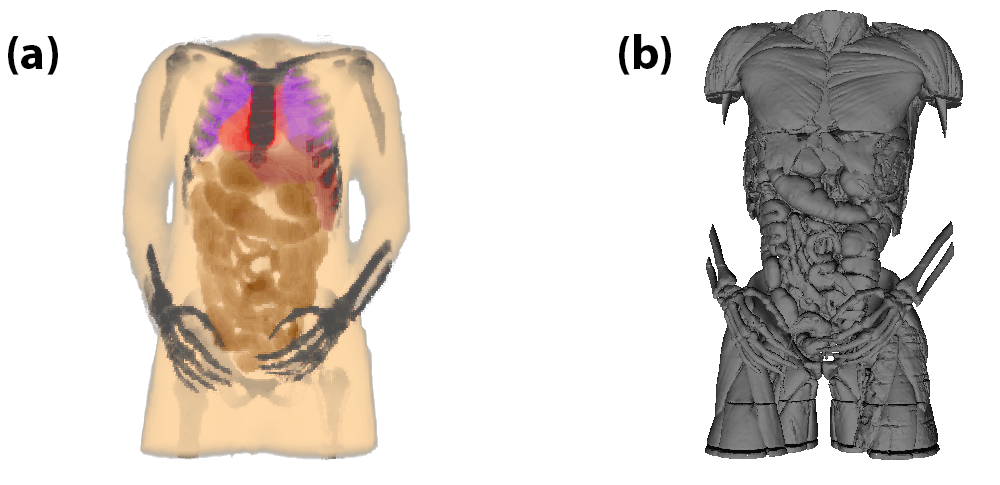
\includegraphics[width=0.5\textwidth]{IMG/volvsb-rep.png}
    \caption{La figura (a) muestra la representación volumétrica del \emph{Visible Human Project}\cite{ackerman1998visible}. La figura (b) muestra la malla poligonal del mismo modelo. }
   \label{fig:HVP}
\end{figure}
\todo{hace falta explciar la malla de tetraedros?}
Una de las necesidades básicas de un simulador para ser realista es que la información anatómica de los pacientes virtuales con las que trabajará el usuario sean realistas. Para ello se necesita seleccionar un modelo anatómico realista en alguna representación anteriormente comentada. Además, también se busca que la experiencia sea lo más cercana a la realidad posible y a la vez que contemple una gran variedad de casos. En  \cite{preim2018survey} se explica la necesidad de que los estudiantes tengan un conocimiento profundo de la anatomía humana, estructuras, su posición relativa, variabilidad, etc... En este artículo se presenta un resumen de técnicas de visualización e interacción desarrolladas para este fin.

Respecto a los modelos humanos virtuales, existen varios modelos comerciales como puede ser \emph{ZygoteBody}$^{TM}$ ~\cite{kelc2012zygote}, \emph{Anatomium} ~\cite{Anatomium},   \emph{BioDigital Human} \cite{qualter2012biodigital}o modelos como \emph{Visible body}\cite{visible2012visible} que solo está centrado en músculos y deformaciones predefinidas. Estos modelos han sido  diseñados por artistas representan cánones no realistas que no reflejan fielmente la anatomía de los pacientes a las que podría enfrentarse un médico. Para ello, en la actualidad se sigue investigando para llevar datos de pacientes reales a modelos virtuales y de esta forma usar datos capturados usando técnicas de imagen médica (como CT, MRI o US). Existen incluso representaciones volumétricas casi completas como son el \emph{Visible Human Project}\cite{ackerman1998visible}  y un modelo basado en este llamado \emph{Segmented Inner Organs}\cite{VoxelMan}. Sobre estos datos capturados, muchos investigadores han propuesto métodos para llevar esto acabo y se pueden consultar \cite{ferrante2017slice}.

Tanto los modelos comerciales como los modelos obtenidos a través de imagen médica, presentan el mismo problema: los modelos son presentados en una misma postura, que suele coincidir con la postura de adquisición. Esto hace que los datos de pacientes sean estáticos y limitados que no representan la mayoría de los casos. Es en algunos procedimientos médicos como puede ser la artroscopia de rodilla, las imágenes capturadas no presentan la misma postura que será necesaria para el procedimiento adecuado, ya que se necesita la rodilla flexionada frente a la pierna extendida donde fue capturada la imagen. 

Es importante remarcar que la mayoría de las técnicas que se presentan en \cite{ferrante2017slice} no son capaces de capturar adecuadamente todos y cada uno de los tejidos del paciente. En ocasiones solo se centran en tejidos concretos como puede ser la piel y músculos en general. Además, las técnicas actuales de imagen médica tampoco son capaces de recuperar las propiedades mecánicas de todos los tejidos siendo esto un gran inconveniente al intentar simular fielmente estos datos.

Por tanto, estos simuladores necesitaran un método que pueda tratar datos de personas con todos los tejidos internos, de esta manera se podrá reproducir todo tipo de posturas, posiciones y, en resumen, generar variabilidad para que los usuarios puedan entrenar un gran número de posibilidades en los simuladores médicos.




\subsection{Animación de personajes} 
\label{art:animation}

En esta sección se presentan una visión general de los diferentes algoritmos existentes para animar modelos tridimensionales. La animación consiste en deformar la representación B-rep o volumétrica por medio de modelos matemáticos. Estos modelos matemáticos pueden ser clasificados de dos tipos, aquellos que tienen en cuenta las propiedades físicas del modelo y aquellos que solo utilizan operaciones geométricas para animar el modelo. Actualmente, es habitual que los algoritmos geométricos esta orientados a ser interactivos sacrificando deformaciones físicamente correctas y los algoritmos físicos están centrados en una deformación más realista.  Aun así, existen algoritmos que combinan ambos enfoques para conseguir deformaciones más realistas con tasas interactivas, o reducir el tiempo de procesado mientras se mantiene el comportamiento físico. 


\subsection{Animación esqueletal}
\label{art:virtualskel}

La animación esqueletal es un método geométrico que anima un modelo representado por su malla superficial, normalmente llamada piel, y un esqueleto virtual formado por huesos ordenados jerárquicamente. Asociando los vértices a los distintos huesos, esta técnica permite transferir el movimiento del esqueleto a su piel. Esta técnica fue introducida por Nadia Magnenat en 1988 \cite{thalmann88} y sigue siendo la técnica más utilizada debido a su sencillez y su fácil adaptación al cauce gráfico. A pesar de la existencia de métodos más realistas, esta técnica se usa prácticamente en todos los sistemas de animación ya que simplifica el trabajo de los artistas o es el paso previo a algoritmos más complejos. Por ejemplo, se puede animar mediante captura de movimientos y cinemática inversa entre otros.

the virtual skeleton is a mathematical
abstraction used to define the rotation point of the different VPH model joints.
These rotation points are called virtual joints and they are hierarchically
structured.
Magnenat-Thalmann et al in their seminal paper [1] describe how virtual
skeletons can be applied to animate 3D meshes. Figure 3 shows an example
of a virtual skeleton superimpose to the virtual patient bones and skin. The
grey spheres represent the virtual joints, while the grey prisms represent the
hierarchical relationship among the virtual joints.

\begin{figure}[h]
   \centering
    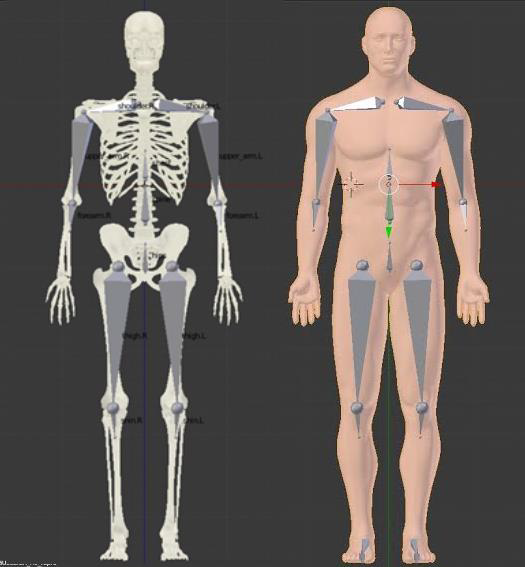
\includegraphics[width=0.5\textwidth]{IMG/virtualskeleton.png}
    \caption{ }
   \label{fig:zygoteproblems}
\end{figure}

Con el paso del tiempo, se han definido los siguientes conceptos en los que se puede dividir la animación esqueletal:

\begin{itemize}
    \item \emph{Rigging}\footnote{Término utilizado en la industria para la creación o adaptación del esqueleto virtual \label{footnote1}}: En esta etapa se crea el esqueleto virtual específicamente para el modelo que queramos animar
    \item Pesado: Una vez creados los huesos virtuales, se asigna el peso de influencia de cada hueso para cada vértice de la piel del modelo.
    \item \emph{Skinning}\textsuperscript{\ref{footnote1}}: Se define las operaciones matemáticas que van a transferir el movimiento de los huesos 
    \item Animación: Se mueven los huesos y esto produce una deformación en la piel.
\end{itemize}

A continuación se mostrará la revisión de la literatura existente para cada etapa.
\subsubsection{Rigging}
\label{art:rigging}

El proceso de \emph{rigging} consiste en crear un esqueleto virtual lo más cercano a el esqueleto original que tuviera el modelo tridimensional que se esta animando. Este trabajo normalmente es realizado por un artista ayudado de un programa CAD (siglas en ingles de diseño asistido por computador) como puede ser \emph{Blender} \cite{a}, herramientas de \emph{Autodesk} como pueden ser \emph{Maya} o \emph{3DS MAX} \cite{a}. También existen algunos trabajos que tratan de automatizar el proceso de creación de esqueletos virtuales siguiendo dos enfoques: adaptando esqueleto predefinido \cite{a} o infiriendo el esqueleto en base a la malla superficial \cite{a}.
Existen limitaciones para aquellos esqueletos virtuales que solo se definen por rotaciones, ya que los movimientos de modelos orgánicos son mucho más complejos. Algunos trabajos intentan definir articulaciones basado en modelos anatómicos \cite{joints} con \emph{splines}\footnote{ es una curva diferenciable definida en porciones mediante polinomios} mejorando el movimiento del hueso pero dificultando la creación del esqueleto virtual y el proceso de manipulación.
Currently, there exist several techniques to adapt a generic virtual skeleton to a 3D character~\cite{huang2013robust,feng2014fast,pan2017automatic}.


\subsubsection{Pesado}
\label{art:pesado}

Este proceso  determina cual es la influencia de cada hueso virtual en cada vértice de la malla superficial. El cálculo de esta influencia se denomina pesado al determinar que un vértice lleva asociado una serie de pesos $w_{i,j}$ que relacionan un vértice $i$ con el hueso $j$.
Para asegurar una deformación correcta se presuponen las siguientes condiciones que tienen que cumplir el pesado:
\begin{eqnarray}
%\begin{equation}
\label{cond1}
w_{i,j}\geq 0 \;\;\;\;\;\;\;\; \forall i \in V \wedge \forall j \in B   \\
%\end{equation}
%\begin{equation}
\label{cond2}
\sum_{j \in B} w_{i,j} = 1\ \;\;\;\;\;\;\;\;\;\;\;\;\;\;\;\;
\forall i \in V
%\end{equation}
\end{eqnarray}
Donde V es el conjunto de vértices de la malla poligonal y B son el conjunto de huesos en el esqueleto virtual. No puede existir un hueso que influya negativamente a un vértice, por ello se tiene que cumplir la condición \ref{cond1}. Además, para garantizar que no se genere movimientos extra, es necesario cumplir la condición \ref{cond2}.
Por último, resulta intuitivo pensar que las transiciones entre huesos virtuales deberían ser progresivas, el gradiente de los pesos debe ser suave, para evitar efectos extraños y discontinuidades en la malla.

Originalmente, al igual que la etapa anterior, un artista era el encargado de realizar la tarea manualmente, donde se utilizaban herramientas \emph{CAD} para \emph{pintar} la influencia de un hueso en la malla superficial. Actualmente en la literatura se pueden encontrar métodos semi-automáticos\cite{a} y también totalmente automáticos \cite{}. 
Algunos de estos trabajos no tienen en cuenta la conectividad de la malla y puede ser que haya vértices topológicamente lejanos con pesos similares. Se han propuesto soluciones como \cite{Baran:2007} utilizando ecuaciones diferenciales que ayudan a calcular transiciones más suaves en la malla. Esta solución es más compleja (resolución de sistemas de ecuaciones, cálculo de vecindad, etc) pero ofrece transiciones más realistas y menor intervención manual.

explain the properties the weights $w_{i,j}$ must meet: (i) the vertex weights must be independent of the mesh topology or resolution; (ii) the weights must vary smoothly along the volume. In order to ensure these two properties, they proposed to use Laplace diffusion equation.

\emph{Baran and Popovi\'{c}}~\cite{Baran:2007} propose an algorithm to automate both rigging and weighting stages. In their work, they adapt a previous generated virtual skeleton to a 3D model. Then, the influences of the virtual bones over the vertex of the surface mesh are computed using Laplace diffusion equation. This technique is constrained to B-Rep models and the surface mesh must completely enclose the virtual skeleton. 
The weighting phase of our animation pipeline extends this technique to deal with the internal anatomy of the model and to take into account the models’ bone tissue for building the virtual skeleton.
\emph{Baran and Popovi\'{c}}~\cite{Baran:2007} propose an algorithm to automate both rigging and weighting stages. In their work, they adapt a previous generated virtual skeleton to a 3D model. Then, the influences of the virtual bones over the vertex of the surface mesh are computed using Laplace diffusion equation. This technique is constrained to B-Rep models and the surface mesh must completely enclose the virtual skeleton. 
The weighting phase of our animation pipeline extends this technique to deal with the internal anatomy of the model and to take into account the models’ bone tissue for building the virtual skeleton. 
\emph{Jacobson et al.}~\cite{Jac2011} improve the weighting phase to deal with point handles, virtual bones and cages. They minimize the Laplacian energy subject to the handles' constraints (among other constraints) to achieve high-order smoothness (see equation \ref{eqn:1}):
\begin{equation}
\label{eqn:1}
\mathrm{arg\,min}_{W_j, j=1..m}\sum_{j}^m\frac{1}{2}\int_\Omega \left \|  \nabla W_j\right \|^2 dV,
\end{equation}
where $W_j$ are the weights of the handle $j$ and $m$ is the number of handles. 

\subsubsection{Skinning}
\label{art:skinning}

\subsection{Animación basada en físicas}

%\appendix
%\include{appendix}
\cleardoublepage
% Como incorporar como un capitulo mas en el indice de la bibliografia
\addcontentsline{toc}{chapter}{Bibliografía}

\bibliography{bibliography}
\bibliographystyle{alpha}
\end{document}
